\documentclass[12pt]{article}
\usepackage[letterpaper,margin=.65in,headheight=18pt,headsep=18pt,footskip=25pt]{geometry}
\usepackage[T1]{fontenc}\usepackage{helvet}\renewcommand{\familydefault}{\sfdefault}
\usepackage{tikz,array,fancyhdr}\usetikzlibrary{arrows.meta}
\pagestyle{fancy}\fancyhf{}\renewcommand{\headrulewidth}{0pt}
\fancyhead[L]{\small Week 33 / Necklaces encore / Grades 2--5}
\fancyfoot[L]{\scriptsize Bellingham Math Circle / Week 33 / W33-BON-v1}\fancyfoot[R]{\scriptsize\thepage}
\setlength{\parindent}{0pt}\setlength{\parskip}{9pt}
\newcommand{\problem}[2]{\par\textbf{Problem #1:} #2\par}
\newcommand{\ring}[5]{\begin{tikzpicture}[x=1cm,y=1cm]
\draw[black!35] (0,0) circle (#2);
\foreach \s [count=\i from 0] in {#4}{\coordinate (p) at ({90-360*\i/#1}:#2);\draw[fill=white] (p) circle (#3);\ifnum\pdfstrcmp{\s}{-}=0\else\node[font=\small] at (p){\s};\fi}
\node[anchor=north] at (0,{-#2-#3-.2}){#5};\end{tikzpicture}}
\newcommand{\codecards}[1]{\begin{tikzpicture}[x=1cm,y=1cm]\foreach \s [count=\i from 0] in {#1}{\draw ({mod(\i,4)*2.8},{-floor(\i/4)*1.15}) rectangle +(2.5,.9);\node at ({mod(\i,4)*2.8+1.25},{-floor(\i/4)*1.15+.45}){\s};}\end{tikzpicture}}
\begin{document}
Counter kinds keep their names. Turning a ring may match it to another ring. For Problem 1, test flips with a tracing copy while the original stays still.
\problem{1}{Build and compare these six rings. Group the ring labels when only turns are allowed. Then group them when turns and flips are allowed.}
\begin{center}\begin{tabular}{ccc}
\ring{8}{1.05}{.22}{A,A,B,A,B,B,B,B}{a}&\ring{8}{1.05}{.22}{A,B,B,B,B,A,B,A}{b}&\ring{8}{1.05}{.22}{B,A,A,B,A,B,B,B}{c}\\[6mm]
\ring{8}{1.05}{.22}{A,A,B,B,A,B,B,B}{d}&\ring{8}{1.05}{.22}{A,B,B,B,A,B,B,A}{e}&\ring{8}{1.05}{.22}{B,B,A,A,B,B,A,B}{f}
\end{tabular}\end{center}
Only turns: \hrulefill\par
Turns and flips: \hrulefill
\begin{center}\ring{8}{3.3}{1.2}{-,-,-,-,-,-,-,-}{}\end{center}
\newpage
For the remaining problems, rings stay face up. Only turns count as matches.
\problem{2}{Make each ring using only A and B, with different kinds at every neighboring pair, including the closing pair. Which rings can be made? Explain any impossibility.}
\begin{center}\begin{tabular}{cc}
\ring{4}{2.1}{1.2}{-,-,-,-}{}&\ring{5}{2.4}{1.2}{-,-,-,-,-}{}\\[6mm]
\multicolumn{2}{c}{\ring{6}{2.6}{1.2}{-,-,-,-,-,-}{}}
\end{tabular}\end{center}
\vspace{2cm}
\newpage
\problem{3}{Use A, B, and C to make five-bead rings with different kinds at every neighboring pair. Find every ring. Rings that match by turning count as one; flips do not count as matches.}
\begin{center}\ring{5}{2.4}{1.2}{-,-,-,-,-}{}\end{center}
\begin{center}\begin{tabular}{cccc}
\ring{5}{1.15}{.28}{-,-,-,-,-}{}&\ring{5}{1.15}{.28}{-,-,-,-,-}{}&\ring{5}{1.15}{.28}{-,-,-,-,-}{}&\ring{5}{1.15}{.28}{-,-,-,-,-}{}\\[8mm]
\ring{5}{1.15}{.28}{-,-,-,-,-}{}&\ring{5}{1.15}{.28}{-,-,-,-,-}{}&\ring{5}{1.15}{.28}{-,-,-,-,-}{}&\ring{5}{1.15}{.28}{-,-,-,-,-}{}
\end{tabular}\end{center}
\vspace{2cm}
\newpage
A window reads consecutive beads clockwise. Start at every bead, including windows that cross the closing gap. A removable viewer marks which beads to read. For each test, use a fresh complete deck. Your partner removes one matching card at every start. If it is already gone, the ring fails.
\begin{center}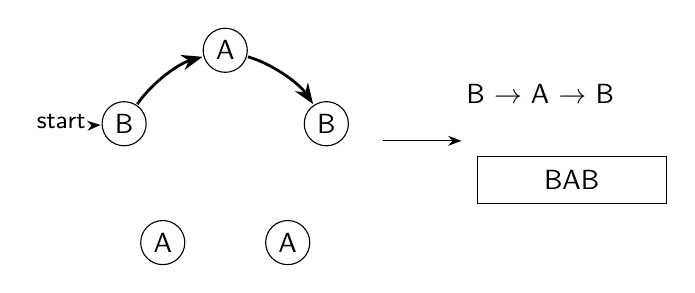
\begin{tikzpicture}[x=1cm,y=1cm,>=Stealth]
\foreach \s [count=\i from 0] in {A,B,A,A,B}{\coordinate (p\i) at ({90-72*\i}:1.35);\draw[fill=white] (p\i) circle (.28);\node at (p\i){\s};}
\draw[->,line width=1pt,shorten >=3mm,shorten <=3mm] (p4) to[bend left=20] (p0);\draw[->,line width=1pt,shorten >=3mm,shorten <=3mm] (p0) to[bend left=20] (p1);
\node[anchor=east,font=\small] at (-1.65,.45){start};\draw[->,shorten >=3mm] (-1.6,.4)--(p4);
\node at (4,.8){B $\to$ A $\to$ B};\draw[->] (2,.2)--(3,.2);
\draw (3.2,-.6) rectangle (5.6,0);\node at (4.4,-.3){BAB};
\end{tikzpicture}\end{center}
\problem{4}{Make the shortest A/B ring that contains each two-letter card exactly once as a window.}
\begin{center}\codecards{AA,AB,BA,BB}\end{center}
\begin{center}\ring{4}{2.1}{1.2}{-,-,-,-}{}\end{center}
\problem{5}{Why can no shorter ring contain all four cards?}
\vspace{2cm}
\newpage
\problem{6}{Make the shortest A/B ring that contains each three-letter card exactly once as a clockwise window.}
\begin{center}\codecards{AAA,AAB,ABA,ABB,BAA,BAB,BBA,BBB}\end{center}
\begin{center}\ring{8}{3.3}{1.2}{-,-,-,-,-,-,-,-}{}\end{center}
\problem{7}{Find every shortest ring for the eight cards. Rings that match by turning count as one. How are their flipped copies related to your collection?}
\begin{center}\begin{tabular}{cc}
\ring{8}{1.1}{.26}{-,-,-,-,-,-,-,-}{}&\ring{8}{1.1}{.26}{-,-,-,-,-,-,-,-}{}
\end{tabular}\end{center}
\end{document}
